\documentclass{beamer}
\usepackage[utf8]{inputenc}

\usetheme{Madrid}
\usecolortheme{default}
\usepackage{amsmath,amssymb,amsfonts,amsthm}
\usepackage{txfonts}
\usepackage{tkz-euclide}
\usepackage{listings}
\usepackage{adjustbox}
\usepackage{array}
\usepackage{tabularx}
\usepackage{gvv}
\usepackage{lmodern}
\usepackage{circuitikz}
\usepackage{tikz}
\usepackage{graphicx}
\usepackage{mathtools}

\setbeamertemplate{page number in head/foot}[totalframumber]

\usepackage{tcolorbox}
\tcbuselibrary{minted,breakable,xparse,skins}



\definecolor{bg}{gray}{0.95}
\DeclareTCBListing{mintedbox}{O{}m!O{}}{%
  breakable=true,
  listing engine=minted,
  listing only,
  minted language=#2,
  minted style=default,
  minted options={%
    linenos,
    gobble=0,
    breaklines=true,
    breakafter=,,
    fontsize=\small,
    numbersep=8pt,
    #1},
  boxsep=0pt,
  left skip=0pt,
  right skip=0pt,
  left=25pt,
  right=0pt,
  top=3pt,
  bottom=3pt,
  arc=5pt,
  leftrule=0pt,
  rightrule=0pt,
  bottomrule=2pt,
  toprule=2pt,
  colback=bg,
  colframe=orange!70,
  enhanced,
  overlay={%
    \begin{tcbclipinterior}
    \fill[orange!20!white] (frame.south west) rectangle ([xshift=20pt]frame.north west);
    \end{tcbclipinterior}},
  #3,
}
\lstset{
    language=C,
    basicstyle=\ttfamily\small,
    keywordstyle=\color{blue},
    stringstyle=\color{orange},
    commentstyle=\color{green!60!black},
    numbers=left,
    numberstyle=\tiny\color{gray},
    breaklines=true,
    showstringspaces=false,
}
%------------------------------------------------------------
%This block of code defines the information to appear in the
%Title page
\title %optional
{5.3.36}
\date{October 2,2025}
%\subtitle{A short story}

\author % (optional)
{EE25BTECH11002 - Achat Parth Kalpesh}



\begin{document}

\frame{\titlepage}

\begin{frame}{Question}
Solve the system of equations
\begin{align}
    \frac{bx}{a} - \frac{ay}{b} + a + b = 0\\
    bx - ay + 2ab = 0 
\end{align}
\end{frame}

\begin{frame}{Solution}
The above equation can be written as
\begin{align}
    \vec{n_1}^\top \vec{x} &= c_1 \\
    \vec{n_2}^\top \vec{x} &= c_2 \\
    \myvec{\vec{n_1}\\ \vec{n_2}}^\top \vec{x} &= \myvec{c_1\\c_2}
\end{align}
 \begin{align}   
     \vec{A} = \myvec{\vec{n_1}\\ \vec{n_2}}^\top \quad
     \vec{b} = \myvec{c_1\\c_2} 
\end{align}
    \begin{align}
    \vec{A} \vec{x} &= \vec{b}\\
    \myvec{\frac{b}{a} & -\frac{a}{b}\\ b & -a} \vec{x} &= \myvec{-a-b\\-2ab}
\end{align}
    \begin{align}
    \vec{A}^\top \vec{A} \neq \vec{I}
\end{align}    
\end{frame}

\begin{frame}{Solution}
Performing row operations:
\begin{align}
\augvec{2}{1}{\frac{b}{a} & -\frac{a}{b} &-a-b\\ b & -a &-2ab}
&\xleftrightarrow[]{R_1 \leftarrow R_1-\frac{R_2}{b}}
\augvec{2}{1}{\frac{b-a}{a} & 0 & a-b\\ b & -a &-2ab}\\
\augvec{2}{1}{\frac{b-a}{a} & 0 & a-b \\ b & -a &-2ab}
&\xleftrightarrow[]{R_2 \leftarrow -\frac{ab}{b-a} R_1 + R_2}
\augvec{2}{1}{\frac{b-a}{a} & 0 & a-b \\ 0 & -a & -ab}\\
\augvec{2}{1}{\frac{b-a}{a} & 0 & a-b \\ 0 & -a & -ab}
&\xleftrightarrow[]{R_2 \leftarrow -\frac{R_2}{a}}
\augvec{2}{1}{\frac{b-a}{a} & 0 & a-b \\ 0 & 1 &  b}\\
\augvec{2}{1}{\frac{b-a}{a} & 0 & a-b \\ 0 & 1 & - b}
&\xleftrightarrow[]{R_1 \leftarrow \frac{a}{b-a} R_1}
\augvec{2}{1}{1 & 0 & -a \\ 0 & 1 &  b}
\end{align}
\end{frame}

\begin{frame}{Solution}
Thus,
\begin{align}
    \vec{x} = \myvec{-a\\b}
\end{align}
\end{frame}

\begin{frame}[fragile]
  \frametitle{C Code}
  \begin{lstlisting}[language=C]
#include <stdio.h>
void solve_system(double A[2][2], double b[2], double* x_sol, double* y_sol) {  // Solve the 2x2 system using Cramer's rule; det(A)
    double determinant = A[0][0] * A[1][1] - A[0][1] * A[1][0];
    // Check if a unique solution exists.
    if (determinant != 0) {// det(Ax)
        double determinant_x = b[0] * A[1][1] - A[0][1] * b[1];
        // det(Ay)
        double determinant_y = A[0][0] * b[1] - b[0] * A[1][0];
        *x_sol = determinant_x / determinant;
        *y_sol = determinant_y / determinant;
    } else {
        // No unique solution, set results to 0 or an error indicator.
        *x_sol = 0;
        *y_sol = 0;
    }
}
  \end{lstlisting}
\end{frame}

\begin{frame}[fragile]
  \frametitle{Python Code}
  \begin{lstlisting}[language=Python]
import numpy as np
import matplotlib.pyplot as plt
import ctypes

lib_path = './solver.so'
solver_lib = ctypes.CDLL(lib_path)
# Define the argument types and return type for the C function
# The function signature is: void solve_system(double A[2][2], double b[2], double* x, double* y)
solve_func = solver_lib.solve_system
solve_func.argtypes = [
    np.ctypeslib.ndpointer(dtype=np.float64, ndim=2, shape=(2,2)),
    np.ctypeslib.ndpointer(dtype=np.float64, ndim=1, shape=(2,)),
    ctypes.POINTER(ctypes.c_double),
    ctypes.POINTER(ctypes.c_double)
]
solve_func.restype = None
  \end{lstlisting}
\end{frame}

\begin{frame}[fragile]
  \frametitle{Python Code}
  \begin{lstlisting}[language=Python]
# Define the coefficient matrix A and the constant vector b
# 2x - y = 10
# 3x + y = 5
A = np.array([[1, -1],
              [1,  1]], dtype=np.float64)
b = np.array([0, -2], dtype=np.float64)

# Create C-compatible variables to store the results
x_intersect_c = ctypes.c_double()
y_intersect_c = ctypes.c_double()

# Call the C function
solve_func(A, b, ctypes.byref(x_intersect_c), ctypes.byref(y_intersect_c))

# Get the Python values from the C types
x_intersect = x_intersect_c.value
y_intersect = y_intersect_c.value
   \end{lstlisting}
\end{frame}

\begin{frame}[fragile]
  \frametitle{Python Code}
  \begin{lstlisting}[language=Python]
# --- 2. Plot the graph ---

# Generate a range of x values for plotting the lines
x_vals = np.linspace(x_intersect - 10, x_intersect + 10, 400)

# Calculate y values for each equation
# Eq1: 2x - y = 10  => y = 2x - 10
y1_vals =  x_vals
# Eq2: 3x + y = 5   => y = 5 - 3x
y2_vals =  - x_vals -2

# Create the plot
plt.figure(figsize=(10, 10))
plt.plot(x_vals, y1_vals, color='blue')
plt.plot(x_vals, y2_vals, color='green')
   \end{lstlisting}
\end{frame}


\begin{frame}[fragile]
  \frametitle{Python Code}
  \begin{lstlisting}[language=Python]
# Mark and label the intersection point
plt.plot(x_intersect, y_intersect, 'ro', markersize=8)
plt.text(x_intersect + 1.0, y_intersect, f'({x_intersect:.2f}, {y_intersect:.2f})', fontsize=12, va='center')

# --- 3. Add non-overlapping labels directly to the lines ---

# Position the labels on the lines at specific points for clarity
plt.text(4, 2.5, 'x-y=0', color='blue', va='center', ha='left', fontsize=11)
plt.text(-6, 2.5, 'x+y=-2', color='green', va='center', ha='center', fontsize=11)
   \end{lstlisting}
\end{frame}

\begin{frame}[fragile]
  \frametitle{Python Code}
  \begin{lstlisting}[language=Python]
# --- 4. Style the plot ---

plt.title('Solution of the System of Linear Equations for a=1,b=-1')
plt.xlabel('X-axis')
plt.ylabel('Y-axis')
plt.axhline(0, color='black', linewidth=0.5)
plt.axvline(0, color='black', linewidth=0.5)
plt.grid(True, which='both', linestyle='--', linewidth=0.5)
# Set axis limits to better match the example image
plt.xlim(-15, 15)
plt.ylim(-20, 20)
plt.axis('equal') # Ensure aspect ratio is equal
plt.show()
   \end{lstlisting}
\end{frame}


\begin{frame}{Plot}
  \begin{figure}
    \centering
    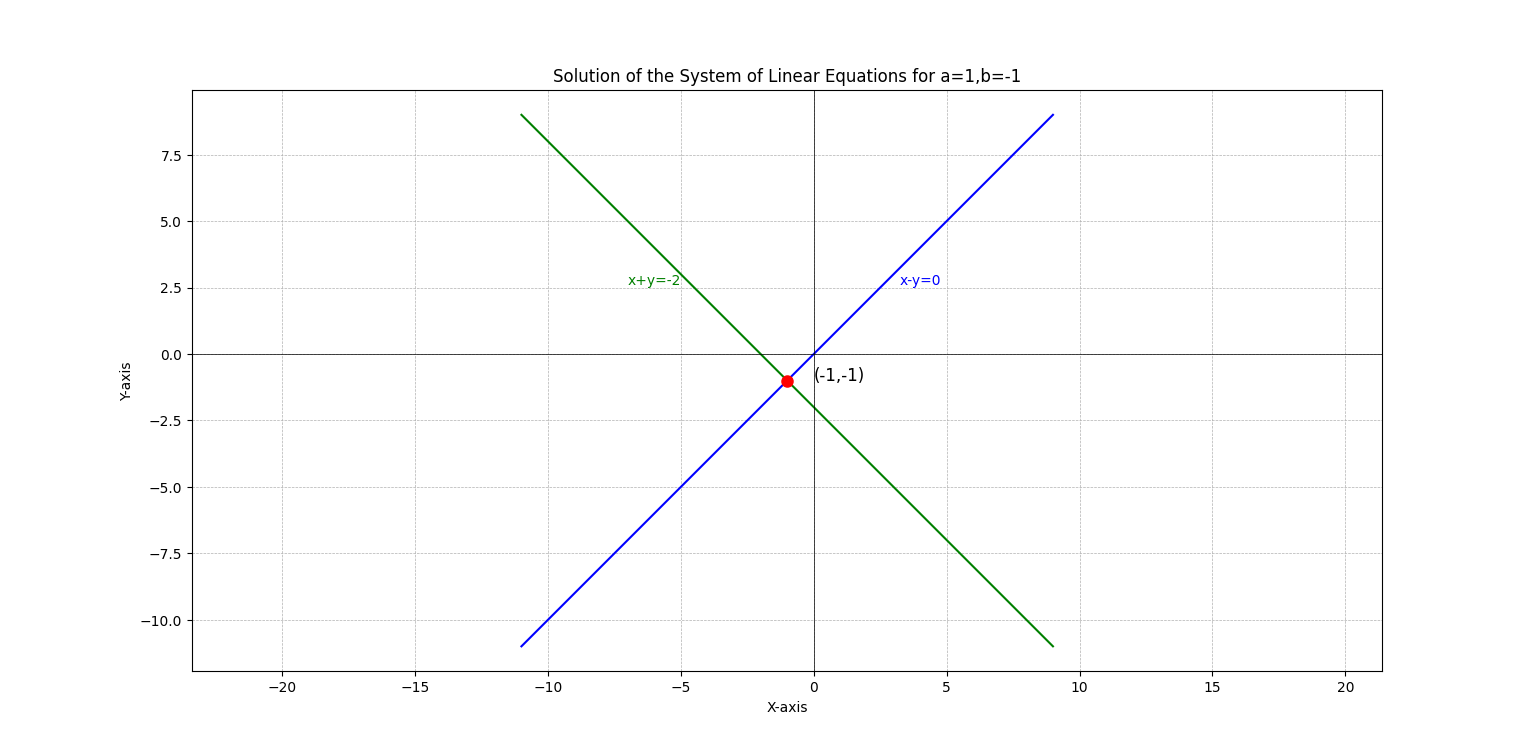
\includegraphics[width=\textwidth]{../figs/figure_py.png}
    \caption{Visualization of the solution}
    \label{fig:final_plot}
  \end{figure}
\end{frame}

\end{document}
